\documentclass{standalone}

\begin{document}

\begin{minted}{python}
def sph2pixel(theta, phi, res=[256,256]):
    x = np.rint((res[0]-1)*wrap(phi)/2/np.pi)
    y = np.rint((res[1]-1)*(1-np.sin(theta))/2)
    return np.array([x, y]).astype(int)

def pixel2sph(x, y, res=[256,256]):
    # phi \in [0, 2*pi]
    # theta \in [-pi/2, pi/2]
    phi = 2*np.pi*x/(res[0]-1)
    theta = np.arccos(2*y/(res[1]-1)-1)-np.pi/2
    return np.array([theta, phi])
\end{minted}

\begin{figure*}
  \caption{\label{fig:imgbuild}
    Illustration marking intermediary steps during the image forming process.
    First, new image is first created as a black canvas.
    Then, during execution the algorithm used by \python{apply\_lensing} iterates through each pixel of the newly generated image and uses the passed lensing map to determine which pixel from the input should be placed at that location.
}
  \begin{tikzpicture}[>=stealth,line width=3pt]
    \tikzset{every node/.style={inner sep=0pt}}
    \def\voffset{3.75cm}
    \def\hoffset{5cm}
    \node (in) at (-\hoffset,0pt)
      {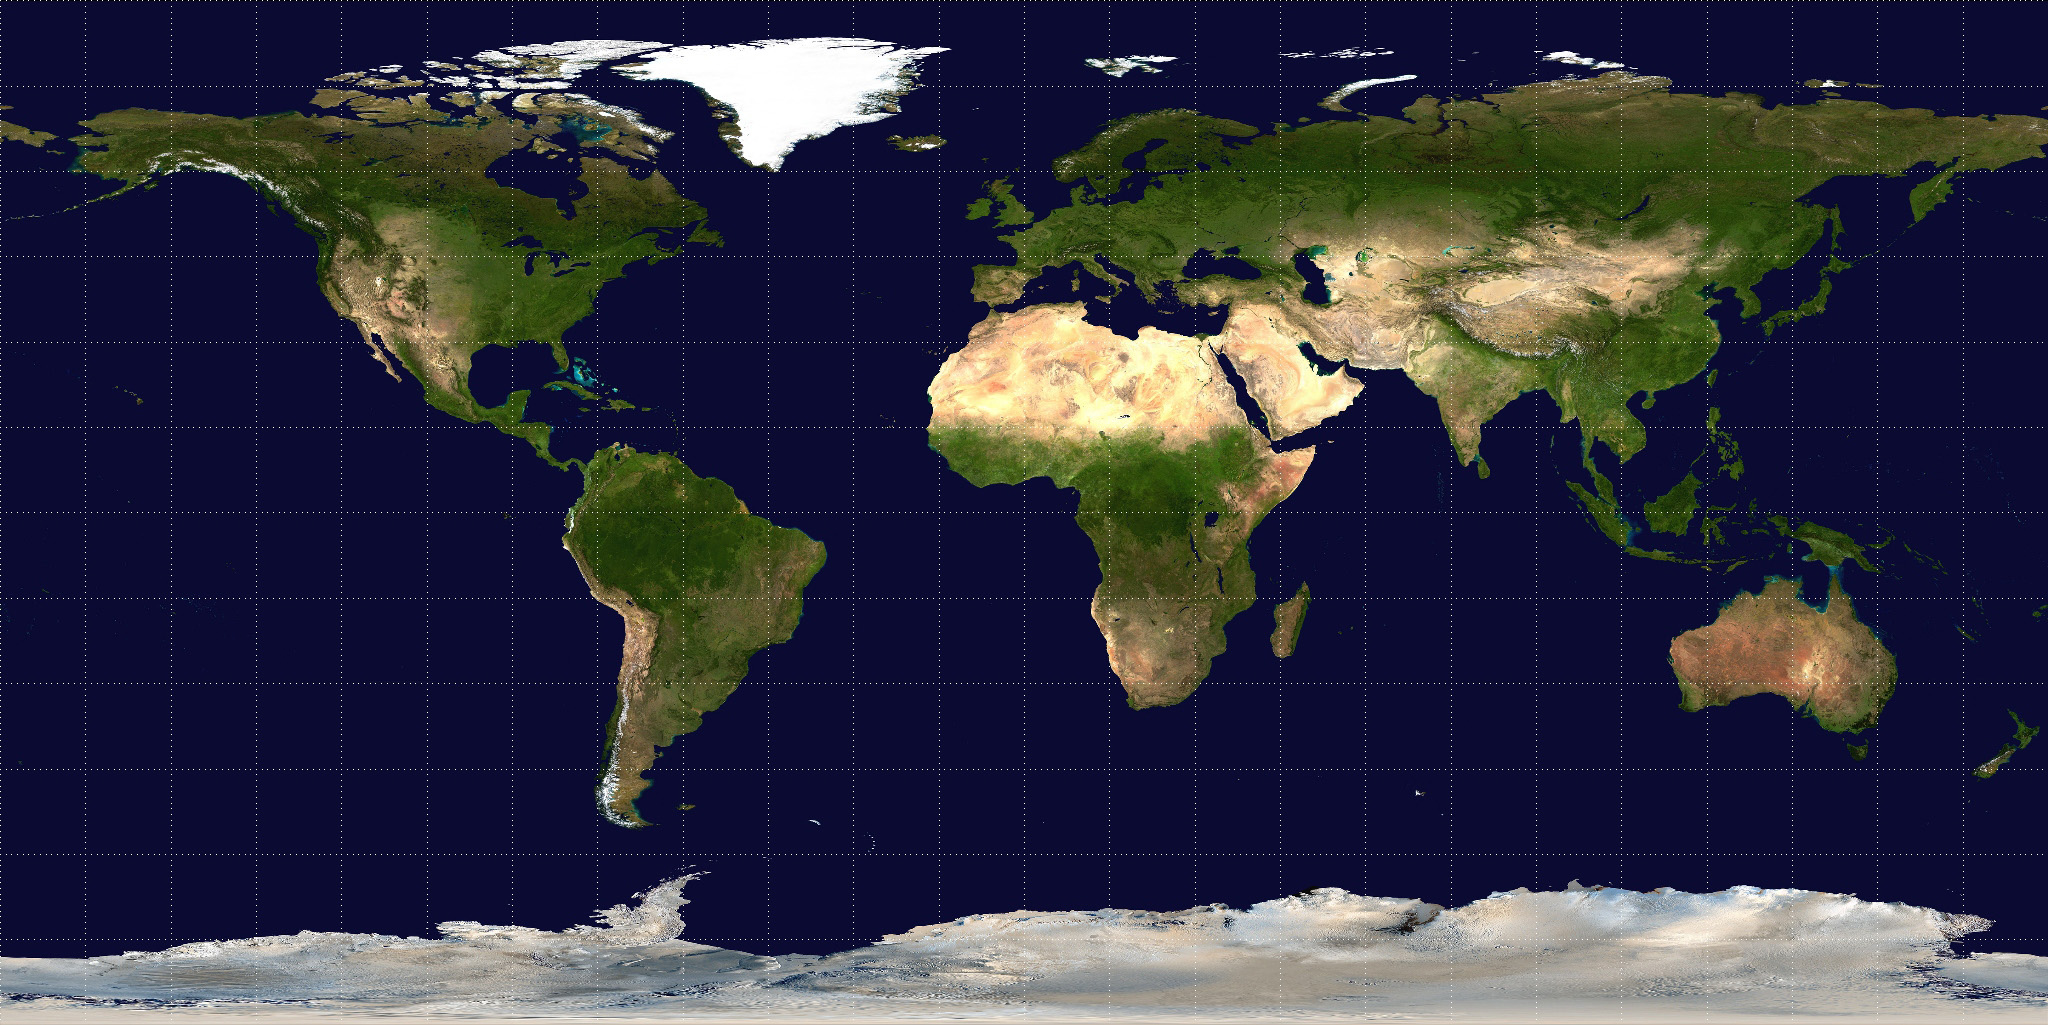
\includegraphics[width=.4\textwidth]{earth}};
    \node (out1) at (\hoffset,\voffset)
      {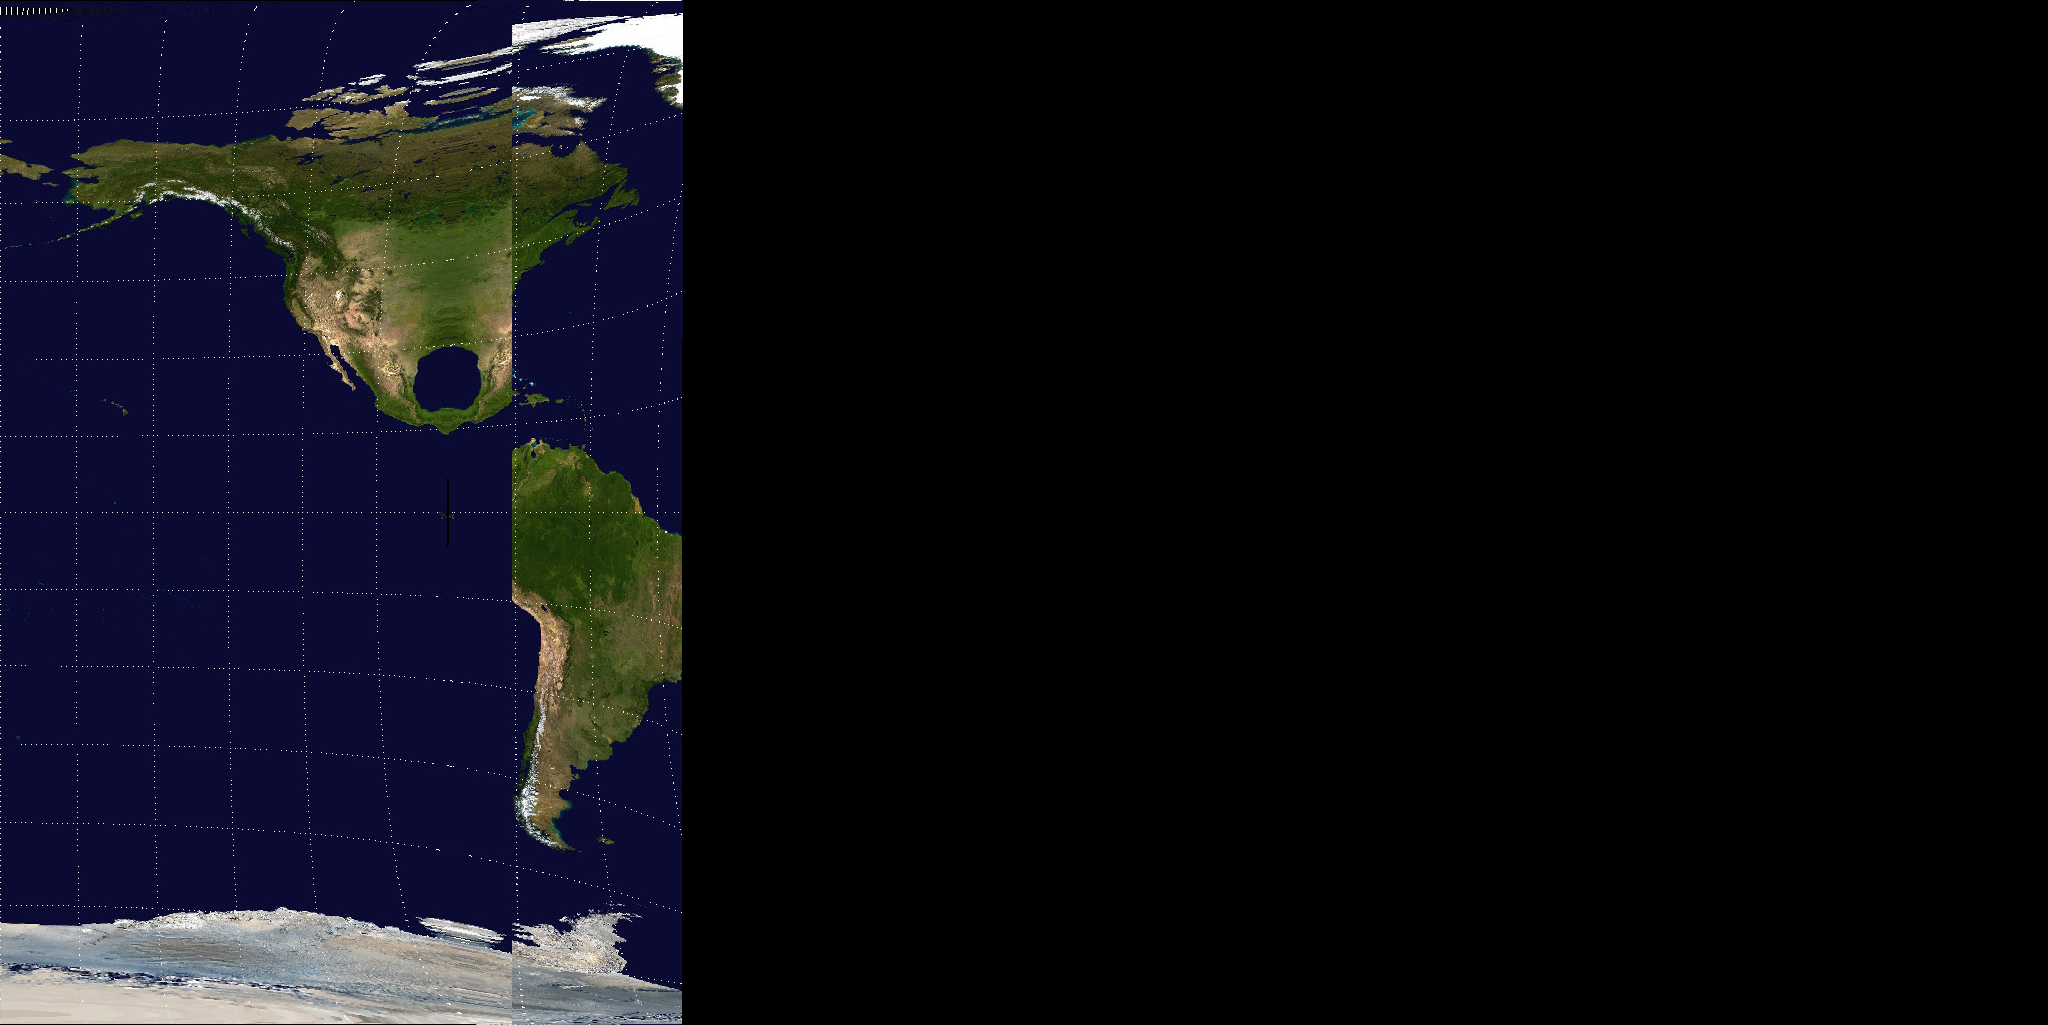
\includegraphics[width=.35\textwidth]{output_onethird}};
    \node (out2) at (\hoffset,0pt)
      {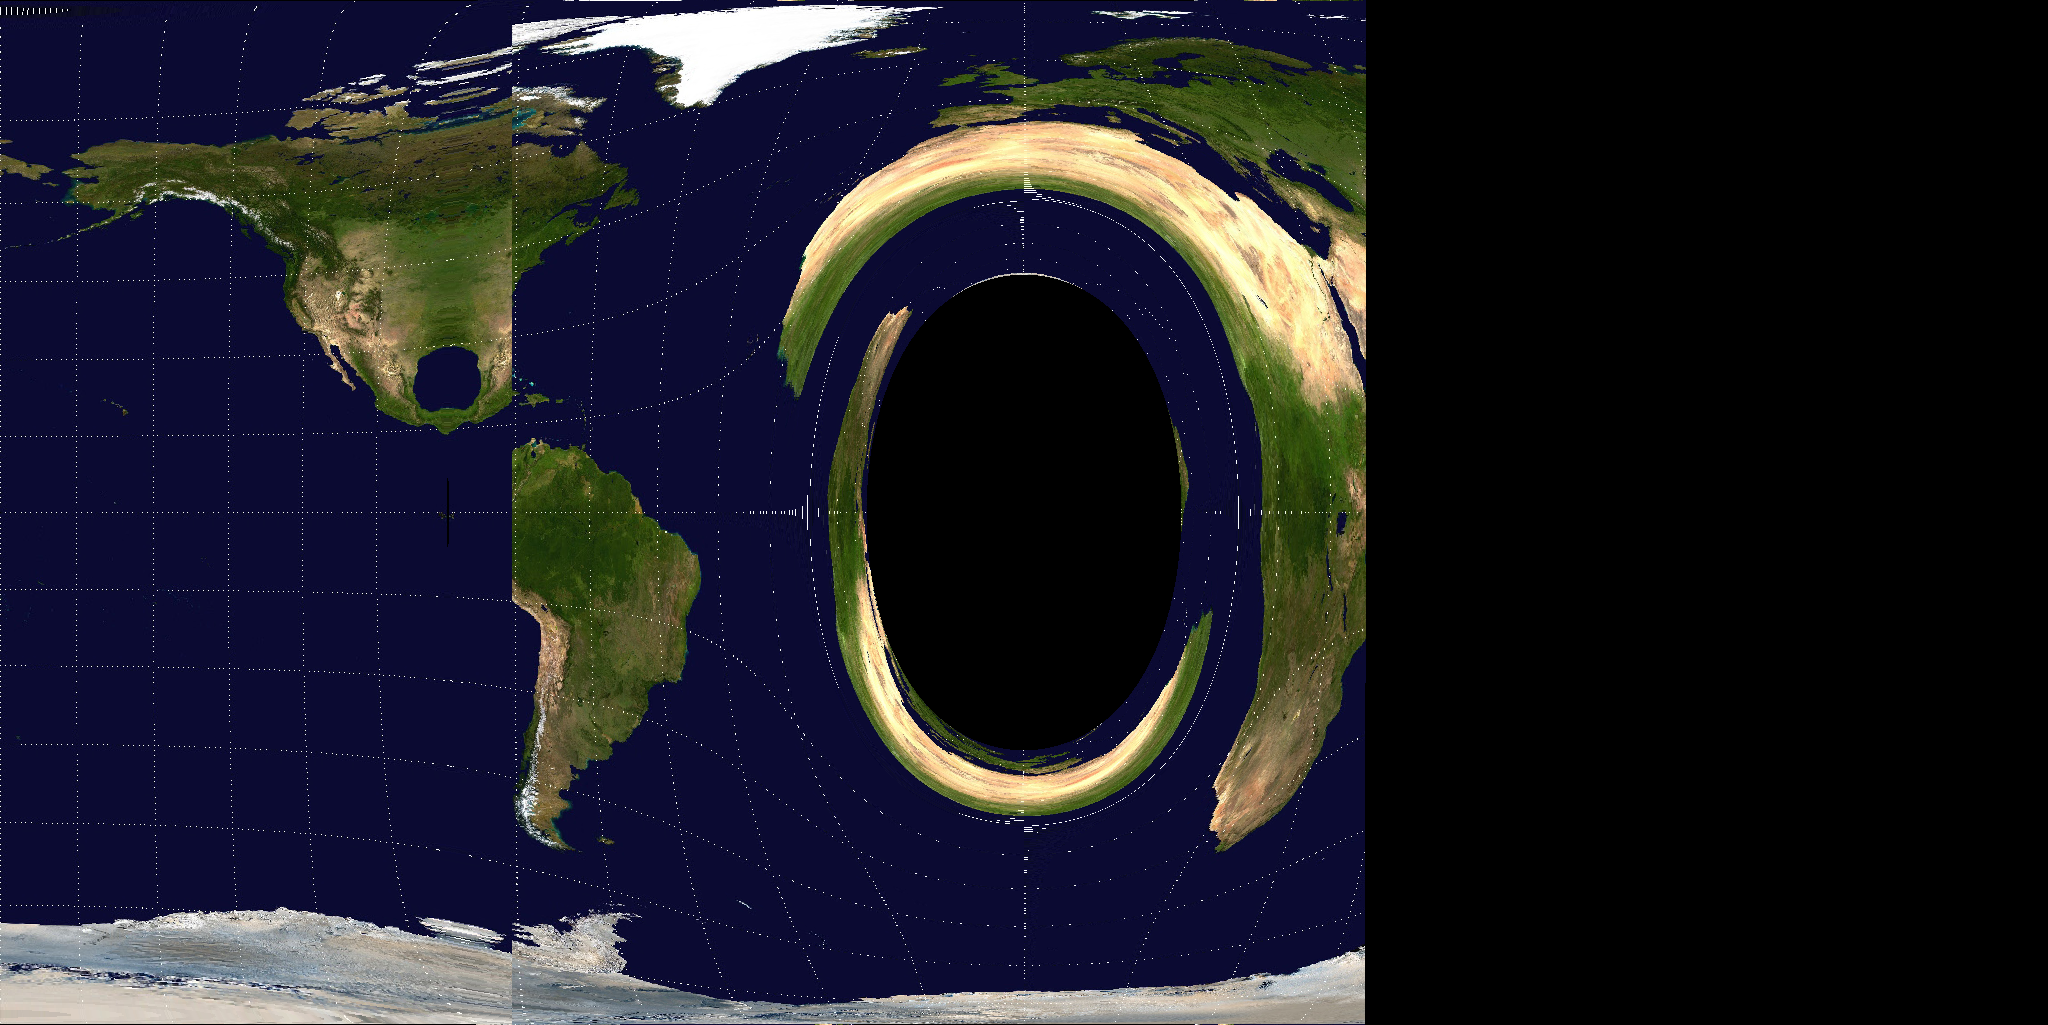
\includegraphics[width=.35\textwidth]{output_twothird}};
    \node (out3) at (\hoffset,-\voffset)
      {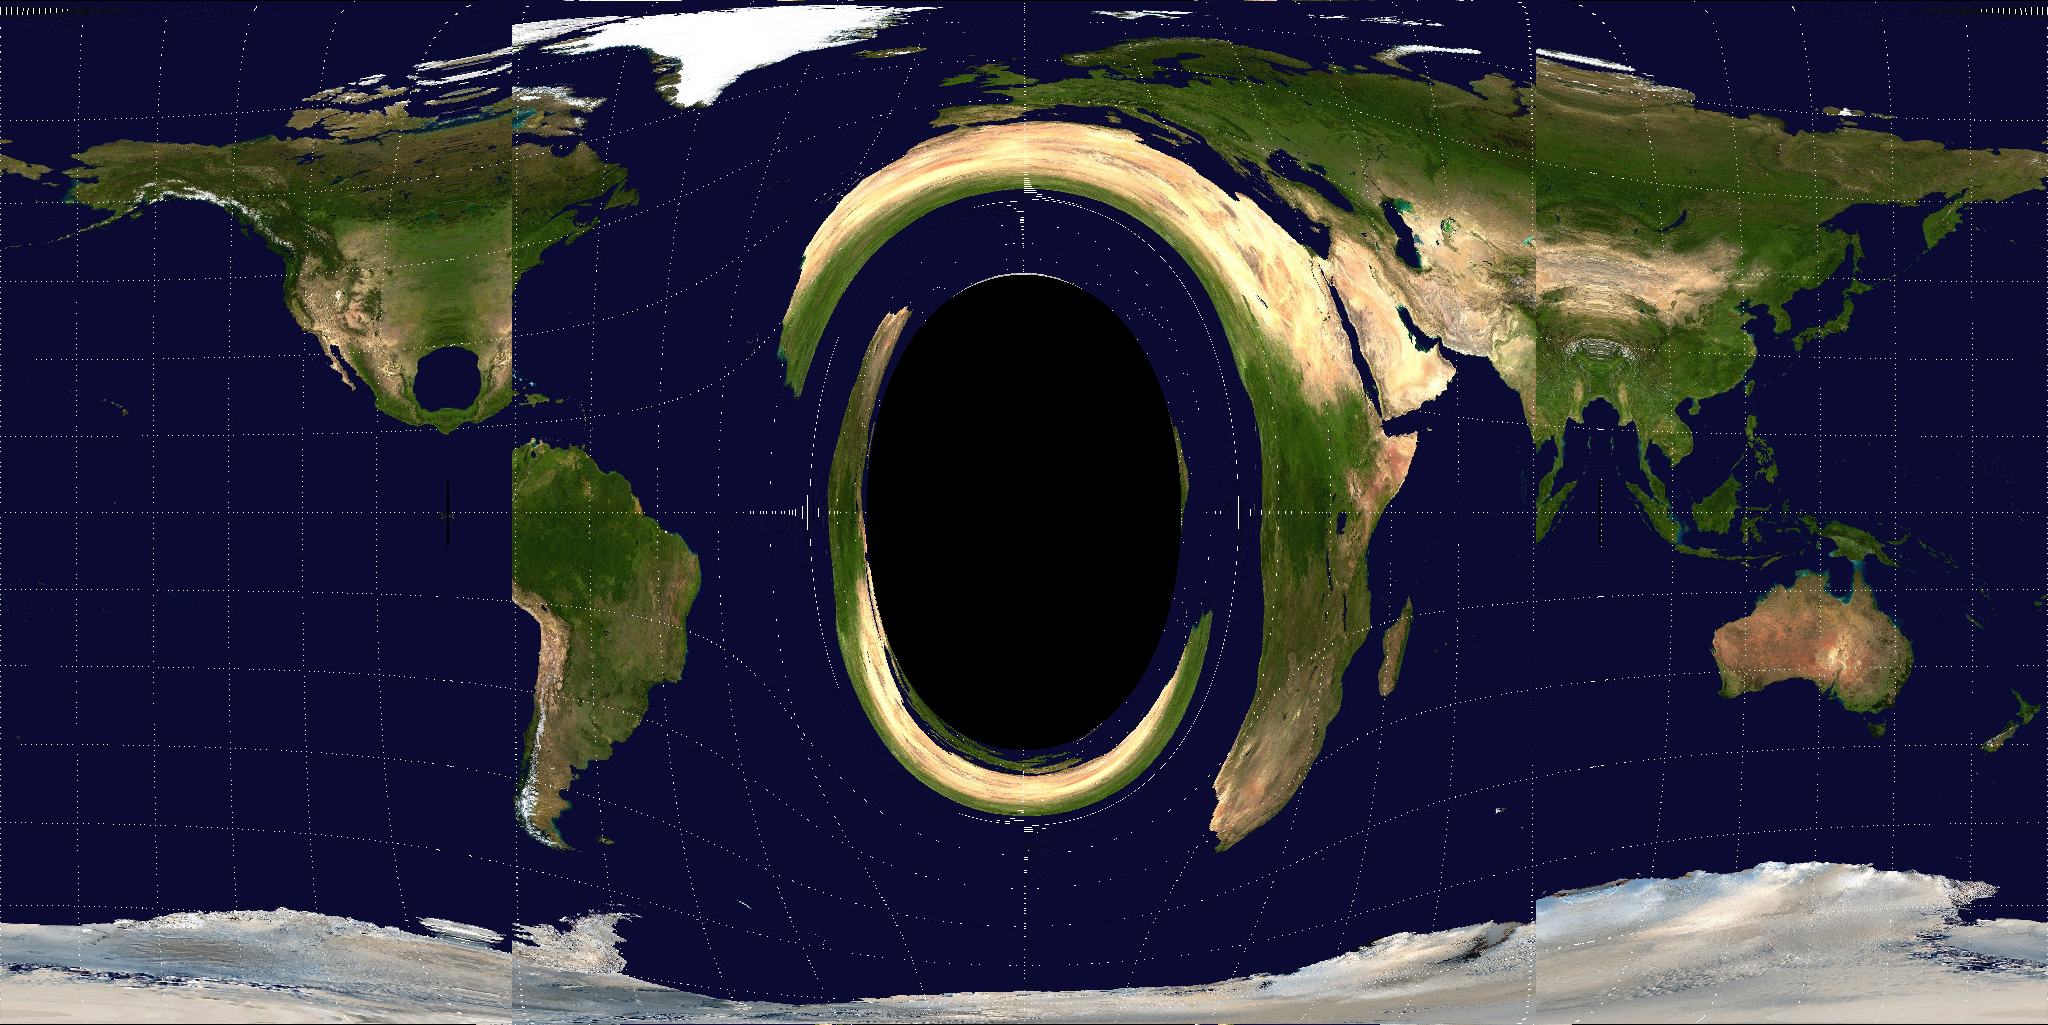
\includegraphics[width=.35\textwidth]{output_full}};
    \draw[->,shorten <=5mm,shorten >=5mm] (in) -- (out2);
    \draw[->] (out1) -- (out2);
    \draw[->] (out2) -- (out3);
  \end{tikzpicture}
\end{figure*}

\end{document}
